%%%%%%%%%%
% LaTeX Problem Set Template
% CISC 203: Discrete Mathematics for Computing II
% Queen's University, Fall 2020
% 
% New TeXnicians:
% Please read the comments below (the lines starting with %)
% and fill in the blanks where a comment reads ``TODO''.
% 
% Template created by Taylor J. Smith (tsmith@cs.queensu.ca).
% Need help? Feel free to get in touch.
% 
% A great resource for help is the LaTeX Stack Exchange:
% https://tex.stackexchange.com
% 
% Also check out Detexify to identify commands for mathematical symbols:
% https://detexify.kirelabs.org/classify.html
%%%%%%%%%%

\documentclass{article}

%%%%%%%%%%
% YOUR INFO
%%%%%%%%%%

% TODO: ENTER YOUR NAME AND THE PROBLEM SET NUMBER HERE
\newcommand{\MyName}{Taylor J. Smith}
\newcommand{\PSNumber}{1}

%%%%%%%%%%
% Packages
%%%%%%%%%%

% These packages let you use math symbols and other related math commands.
\usepackage{amsmath, amssymb, amsthm}

% This package sets the page margins to be 1in all around, giving you more room for beautifully-typeset solutions.
\usepackage[margin=1in]{geometry}

% This package and the following commands set the style of the page headers.
\usepackage{fancyhdr}
\pagestyle{fancy}
\fancyhead[L]{\MyName}
\fancyhead[C]{CISC 203 Problem Set \PSNumber}
\fancyhead[R]{Page \thepage}
\fancyfoot{}
\fancypagestyle{firstpage}{%
    \fancyhf{}
}

% This package allows you to include images in your document.
\usepackage{graphicx}

% Add any other packages you might need here.
%\usepackage{}
\usepackage{xcolor} % This package makes it easier to use colours

%%%%%%%%%%
% Metadata
%%%%%%%%%%

% These commands format the title at the top of page 1. No need to change these.
\title{CISC 203 Problem Set \PSNumber}
\author{\MyName}
\date{\today}

%%%%%%%%%%
% Custom commands
%%%%%%%%%%

% Multiset notation
\def\multiset#1#2{\ensuremath{\left(\kern-.3em\left(\genfrac{}{}{0pt}{}{#1}{#2}\right)\kern-.3em\right)}}

%%%%%%%%%%
% Document
%%%%%%%%%%

\begin{document}

% This command prints the title at the top of page 1.
\maketitle

% TODO: PUT ALL YOUR ANSWERS BELOW
\begin{enumerate}
    % Single-part question format.
    \item Put your answer to Question 1 here.
    \\(\,a)\, \text{is true.} If A \subseteq C, \text{ it means all of the elements of A exist in C as well. We can get }\text{A} \cup \text{C} = \text{C. } \\\text{Therefore, when B} \cup \text{C, the result will be the same as A}\cup \text{B }\cup \text{C. }
    \\(\,b)\, \text{is false. For example, A} = \{1, 2\}, \text{B} = \{2, 3\}, \text{ so A} \cup \text{B} = \{1, 2, 3\}, \\\text{then } (\,A \cup B )\, \triangle \text{A} = \{3\} = \text{B} - \text{A}. \text{ Therefore, the statement is wrong.}

    % Multi-part question format.
    % Some examples of text formatting as well.
    \item
    \begin{enumerate}
        \item Put your answer to Question 2(a) here. \textbf{Make sure it's correct!}
        \\ \{(1,1), (2,2), (3,3), (1,2), (2,1)\}
        \\ \{(1,1), (2,2), (3,3), (1,2), (2,1), (2,3)\}

        
        \item Put your answer to Question 2(b) here. \textit{2(b) or not 2(b)?}
    \end{enumerate}
    
    % Some examples of typesetting math.
    \item Put your answer to Question 3 here. Look out for the equation!
    \begin{equation}
        \zeta(s) = \sum_{n = 1}^{\infty} \frac{1}{n^{s}}
    \end{equation}
    Maybe you want some math inline with your text. Well, here you go: $\binom{n}{k} = \binom{n-1}{k} + \binom{n-1}{k-1}$. For multisets, use: $\multiset{n}{k}$.
    \\ \textbf{Answer for Question 3}
    \\(\,a)\,\text{40+60+50-25-30-35+10 = 70}. \\\text{Therefore, 70 students who had to download at least one of the program}. 
    \\(\,b)\,\text{Number of students who take CISC203 or CISC204: 64+42-16 = 90}.
    \\ \text{Number of students belong to neither CISC203 nor CISC204: 100-90 = 10}.

    % An example of inserting an image.
    % You can use the ``scale'' command below to change the image size.
    % To upload images to Overleaf, see:
    % https://www.overleaf.com/learn/how-to/Including_images_on_Overleaf
    \item Put your answer to Question 4 here.
    {\bf \textcolor{red!90!black}{Note: Hand-written solutions to any question that are scanned/embedded as an image will not be marked. We are showing you how to embed images just for your information and in case any future assignments require including a diagram.}}
    
    \begin{center}
        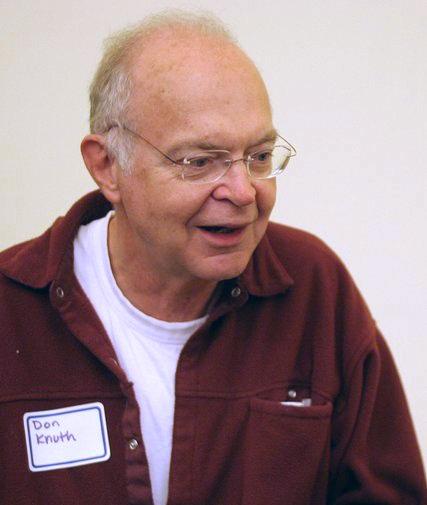
\includegraphics[scale=0.25]{Knuth.jpg}
    \end{center}
    
    % An example of aligning equations using the & symbol.
    % The align environment assigns an equation number to each line, 
    % whereas the align* environment does not.
    % (This also applies to equation vs. equation*)
    \item Put your answer to Question 5 here.
    \begin{align}
        (x+y)^3 &= (x+y)(x+y)(x+y) \\
                &= xxx + xxy + xyx + xyy + yxx + yxy + yyx + yyy \\
                &= x^{3} + 3x^{2}y + 3xy^{2} + y^{3}.
    \end{align}
    
    \begin{align*}
        (x + y)^{n} &=	\sum_{i = 0}^{n} \binom{n}{i} x^{n-i}y^{i} \ \text{(if needed, insert text into your equation environment like so)} \\
		        	&=	\binom{n}{0} x^{n} + \binom{n}{1} x^{n-1}y + \binom{n}{2} x^{n-2}y^{2} + \dots + \binom{n}{n-1} xy^{n-1} + \binom{n}{n} y^{n}.
    \end{align*}
    
    % An example of a ghastly equation, with oversized symbols.
    % Commands like \left( and \right) allow you to nest parentheses and other delimiters, 
    % where the size of the symbol changes based on the surrounding content.
    \item Put your answer to Question 6 here.
    \begin{equation*}
        \left| \bigcup_{k = 1}^{n} A_{k} \right| = \sum_{k = 1}^{n} (-1)^{k+1} \left( \sum_{1 \leq a_{1} < \dots < a_{k} \leq n} \left| \bigcap_{j=1}^{k} A_{a_j} \right| \right).
    \end{equation*}
\end{enumerate}

\end{document}